\subsection{\en{Deep Canonical Correlation Analysis}} \label{DCCA Fundamentals}
\en{Deep Canonical Correlation Analysis is an extension of the standard Canonical Correlation Analysis, created by G. Andrew, R. Arora, J. Bilmes and K. Livescu. As with normal CCA, DCCA is a method that aims to discover and learn associations between two sets of variables. \cite{40}

In the case of DCCA, the method can learn complex, nonlinear relations between the two random vectors and transform them again non-linearly to correlate them, whereas the standard CCA cannot. The method is similar to the idea of Kernel CCA, where the optimal projections are found on the kernel-transformed random vectors, such that the resulting reproducing kernel hilbert space contains the variables in a manner that CCA can be impactful. \cite{41}

However, the problem with KCCA is the computation complexity, as the kernel matrices become very large for real-world datasets, meaning that since it is a nonparametric method, the time required to learn the transformation scales poorly with the size of the data. Additionally, the KCCA method is also limited to the choice of the fixed kernel, meaning they can’t be flexible for different types of datasets. \cite{42}

To address these drawbacks, the use of deep neural networks is proposed, in order to simultaneously learn two deep nonlinear mappings of two random variables. In their paper, they focus on the performance metric of achieved correlation, and comparing it to the correlation of the standard method. \cite{40}

The use of deep learning, meaning neural networks with more than two layers, is designated, since deep neural networks have been proven to be capable of representing accurately and reliably nonlinear functions that model complex real world data.  The method is used to correlate different views of the same dataset, for example different modalities of a biomedical dataset.

The method relies on passing each random vector through a neural network, designed and trained to transform the random vector nonlinearly. That creates a mapping to a hyperspace that results is better correlated to the mapping of the respective (transformed) random vector. 

\newpage
\begin{figure}
    \centering
    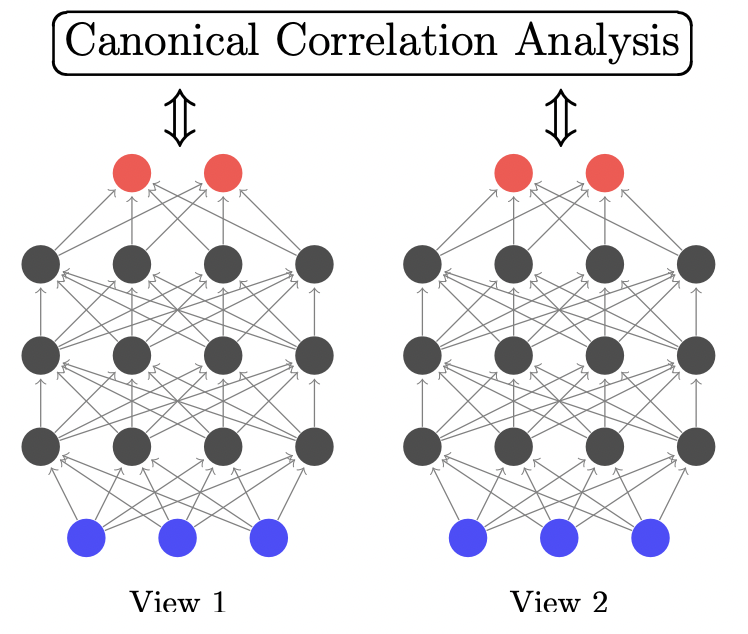
\includegraphics[scale=0.8]{figures/Theoretical_Background/DCCA.png}
    \caption{\en{The two parallel networks, along with the information path (arrows)}}
\end{figure}
\bigbreak

In the figure above, the two neural networks are shown, consisting of 5 layers, with the red layer being the output layer, meaning the vectors that are maximally correlated, and the blue layer being the input layer, meaning the original random vectors. 

If $θ_1$ is the vector of all parameters $(W_i^1, b_i^1)$ of the first network, for each layer i, and respectively $θ_2$ is the vector of all parameters $(W_i^2, b_i^2)$ of the second network for each layer, then the training goal is equivalent to finding the optimum parameters such that the correlation of the output of the networks $f_1(X_1; θ_1), f_2(X_2;θ_2)$ given two random vectors (views) $(X_1, X_2)$. 

That is described as follows:

\bigbreak
$(θ_1^\ast, θ_2^\ast)  = \operatorname{argmax}_{θ_1, θ_2} \{ corr(f_1(X_1; θ_1), f_2(X_2; θ_2))\}$
\bigbreak

Supposing that $H_1,H_2 \in \mathbb{R}^{o\times m}$ are the matrices that contain the respective outputs of the Neural Networks, for each of the  training samples. The target then becomes $corr(H_1, H_2)$. 

To train the networks, the computation of the gradient is needed, and its backpropagation in order to tune the networks parameters. The target is found using the same steps as the standard CCA, while the computation of the gradient, as well as its backpropagation is facilitated through singular value decomposition. 

The authors of the original paper employed full-batch optimization, meaning that before every single weight update step, the network scanned the full dataset. They also used the Limited Memory Broyden–Fletcher–Goldfarb–Shanno (L-BFGS) optimization method. In order to initialise the parameter optimization for the two networks, they utilised a denoising autoencoder for each layer of the networks. The network proposes uses a non-saturating nonlinearity activation function, in the form of:
If $g: \mathbb{R} \to \mathbb{R}$, and $g(x) = {\frac{x^3}{3}} + x$, then the function $s(x) = g^{-1}(x)$ is the activation function, maintaining a sigmoid shape, and unit slope at $x=0$. (\cite{43}, \cite{44})
}